\subsection{Background and motivation}
    % context, setting - B2C business gathers a lot of data
    Many software businesses collect enormous amount of data generated by end-users \cite{chinesemobilebankingusers, bigdatamanagementrevolution, inmon2007tapping}. End-user data incorporates essential information about how users interact with the system of discussion as well as tells a lot about the users themselves \cite{jang2015noreciprocity, hu2014we, jang2016teensengagemorewithfewerphotos, han2016teensarefrommars, socialdiversityongithub}. For instance, such data can explain the preferences of users, what kind of content they like, how they interact with the system and eachother or how frequently they use the software to which their data belongs to \cite{youyou2015computer, ottoni2013ladies}.

    % what is the challenge?
    Depending on the portfolio of the business, analysis of end-user data can reveal various interesting findings. For instance, in banking industry Big Data tools are often used to analyze demographic characteristics to maintain and establish new client relationships \cite{chinesemobilebankingusers, bigdatamanagementrevolution}. Extracting the information from the data is challenging: most businesses are to collect more data than what is humanly possible to process and to analyze \cite{inmon2007tapping, wegener2010integrating}. As a result, significant part of the knowledge might remain unrevealed and hence business-critical information remains unseen \cite{chinesemobilebankingusers, inmon2007tapping, wegener2010integrating, introtodatamining}. 
    
    The computational methods of today's world enable us not only to achieve previously impossible tasks, but also to create tools that may outperform humans \cite{youyou2015computer}. Because of this trait, computational techniques can facilitate our everyday life as well as help us to learn more about the tools and data we work with. Accordingly, there is a growing need for all businesses to introduce data analysis processes in their daily activities with the aim of understanding users and data generated by them better.

    % how do mobile devices have an impact on the amount of data? 
    With the continuous growth of mobile devices in numbers, the amount of data has increased significantly. Due to the wide availability and commonness of smartphones and tablets, anybody can easily generate rich data \cite{jang2016teensengagemorewithfewerphotos}. Complementary to the popularity of mobile devices, social media sites have grown a lot in the recent years \cite{hu2014we, ottoni2013ladies, bakhshi2014faces}, providing users many ways of interaction. Due to the combination of these two trends, users leave digital footprints as location, media, numerical or textual data in numerous places around the Internet \cite{youyou2015computer}. 
    
    People often express their opinion by sharing, liking or commenting on data over social networks. Study shows, that algorithms can predict users' personality traits using such data more reliably than other humans would do \cite{youyou2015computer}. These facts further increase the call for research in the field of user data analysis, because it can help researchers to understand the society, human behavior, preferences and the public's opinion better.

    % what is the potential in analyzing user data? why is it important not only to collect but also analyze data?
    Data analysis tools and methods already exist to facilitate processing user data. However, these applications often not utilized, because companies rather focus on developing their service package over understanding the information gathered in the past \cite{bigdatamanagementrevolution, inmon2007tapping}. It is commonly known, that the utilization of data analysis and Data Mining tools can allow the automatic detection of patterns and interesting relationships in the data \cite{introtodatamining, Friedman97datamining}, which can be a big advantage for businesses in the market. Furthermore, studies show that Knowledge Discovery in Databases is important and is interesting topic in academic research as well \cite{bigdatamanagementrevolution, zarsky2002mine}.
    
    % what is the goal? what is this thesis about?
    The goal of this research is to study the potential use of user data in business and research environments with the application of Data Mining methods. More specifically, one of the goals of this thesis work is to understand what kind of use cases were reported in the relevant literature in this area. In order to do that, the research aims to study how content on the Internet is observed by the users and how users interact with various software solutions which present the information to them. 
    
    Secondly, it is studied what kind of feedback is received from the engaged audience about the presented content in terms of emotional reactions, like activities and comments. Thirdly, the tendencies among the demographic characteristics between users are studied in relation to the content which gets them engaged online. To address these reserach spaces, the Choicely voting/audience engagement platform is taken as a case study. Association analysis, statistical methods and computer vision are utilized to understand the online content and to reveal yet unseen details about the tendencies of user preferences in terms of votes casted on contest participants in the platform. This is done with the aim of improving the quality of service provided by the company so that customers of the firm can analyze the data they have collected from users of the software.
    
    % why is this research conducted, what is the motivation from researcher's pov? 
    One reason behind conducting this research are the stimulating challenges of studying user data and the wide range of possibilities in the information that may lie around in databases. Previous research have proven the relevance of statistical analysis on Big Data, such as like activities \cite{jang2015noreciprocity, jang2016teensengagemorewithfewerphotos, ottoni2013ladies, guy2016whatsyourorganizationlike, jang2015no, youyou2015computer}, user comments \cite{jang2016teensengagemorewithfewerphotos}, image tags \cite{jang2016teensengagemorewithfewerphotos}, image content \cite{hu2014we, bakhshi2014faces} and movie ratings \cite{saraee2004data, kabinsingha2012movie} by revealing interesting findings about user behavior. Moreover, as service providers often get access to user demographics-related data through social network sites in the present time, new possibilities become available to seek correlation between user segments. Studies conducted in this field are also interesting from the point of view of human behavior research, which is another motivation towards conducting studies in this area. 

    % what is the motivation behind the focus from Choicely's point of view? 
    The motivation behind this research from the case company's perspective is mainly oriented towards enhancing the already existing service package that is provided to customers. At the beginning of this research project, the company does not utilize any advanced data analysis tools. This thesis work is motivated in the direction to establish the basis of a Data Mining framework at the company and hence increase the business value of the firm. As the amount of data collected by the company is too large to analyze manually, the application of Data Mining techniques assists the firm and its customers to 

    \begin{itemize}
        \item understand the composition of their active user base better,
        \item have more advanced, quantifiable means on the collected data,
        \item gain an understanding on the users' behavior, 
        \item increase business value by revealing previously unknown patterns.
    \end{itemize} 

\subsection{Research questions, scope and objectives}
In this chapter, the research questions, scope and objectives are presented and explained. The three main research questions are as follows:

    \begin{enumerate}[label=RQ\arabic*:]
        \item \textbf{How is user data understood and utilized in previous research?} The aim of this research question is to discover the conceptual understanding and potential development areas of user data based on related studies. The scope of the concept is defined and it is discussed, how other researchers have studied concept and related areas in the past.
        
        \item \textbf{What kind of content is more engaging for users and draws the most attention in the Choicely platform?} The aim of this research question is to understand which type of voting contests tend to engage a larger audience. Secondly, the question targets to analyze the attributes of those contestants, who received high number of votes. In other words, the aim is to find common features of contestants, who are highly rated by public opinion.

        \item \textbf{What are the behavioral characteristics of users by gender, age and location?} This research question targets to answer the question how users tend to use the platform. This covers the analysis of what kind of content users seek, how the votes are spent and what similarities can be observed in the data. To gain more specific understanding, the users will be grouped by their demographic data.

        %\item \textbf{How is it possible to identify anomalies, such as peaks in or fraud usage from the data?}

        %\item \textbf{How is it possible to recommend relevant content for users based on prior user data?} The question targets to investigate and develop methods which can help users to find new content in the platform relevant to their interests.

        %\item \textbf{What are the privacy concerns to be considered for the case company?}
    \end{enumerate}

    % what is the wide scope of the thesis? What will we begin with as a theoretical background?
    Initially, the study presents an overview on the field of user data analysis in different areas of research as the theoretical part of the study. Particularly, the study addresses the possibilities and challenges of analyses performed on user data in software applications, where users express their opinion via the usage of the system. For example, one can think of like activities on social media, reviewing movies online or voting on their favorite moment of a football match.

    % what is the objective? 
    One of the objectives of this thesis work is to develop advanced data analysis tools in order to assist the case company and its customers to gain a better understanding on the data at hand. In order to do that, the available data is presented and analyzed, the most interesting questions are stated and the information with more influential business value is identified. Afterwards, potential data analysis methods are discussed which are capable to retrieve such information from the given data set. Finally, the behavior of different demographic user groups is studied in the Choicely platform in terms of their activities and what kind of differences can be identified among the different user groups.

    % in what context is this theoretical background relevant? Answer "Why?" % how does that relate to Choicely, particularly? 
    Building on top of the theoretical framework, the study is oriented towards applying techniques for Data Mining purposes at Choicely. Being a large field of science, the scope is focused only on a subset of applicable Data Mining techniques and methods, that are utilized to answer the research questions of this study. Specific topics from the field of Data Science are chosen to obtain the answers to the research questions, such as exploring data, data visualization, association analysis and pattern mining.  

    % what is the focus?
    This research is focused on the challenge of dealing with user data from Computer Science perspective. Although human behavior and psychology experts can benefit from conducting studies in this area, the focus is not shifted to that field of sciences in this work. 

\subsection{Introduction to the Choicely voting platform}
\label{section::introduction-to-the-choicely-voting-platform}
    % what does the company do? 
    Choicely\footnote{\url{http://choicely.com/}} is a voting platform developed by the Finnish Choicely Ltd (formerly known as Lovented Ltd) since 2014. The software provides the possibility for users to engage in interesting contests by voting on their favorite contender. The platform has already hosted numerous contests in various fields, such as beauty pageants, public polls, design contests, talent shows, sport events and many others. The customer base of the firm consist of mainly Finnish broadcasters, publishers, advertisers and beauty pageant organizers. On top of the core customer base in Finland, the recent years have brought numerous users and customers from all around the world. 
    
    The platform is able to host any kind of visual contests or poll. There can be arbitrary number of participants in the contests. Participants must have at least one image and a name attached to them in order to enter the contest. The participants are added by the contest's organizer. 

    % how can one reach a contest in the platform?
    Users can access contests through multiple interfaces (Figure \ref{choicely_platforms}). Naturally, the company's webpage provides a convenient way to create, browse and vote in contests. Choicely also has free mobile applications available on Android and iOS devices, that can be installed through the Google Play\footnote{\url{https://play.google.com/store/apps/details?id=com.choicely.android}} and the iOS App Store\footnote{\url{https://itunes.apple.com/fi/app/choicely/id1158798364}} to the devices. 
    
    \begin{figure}[h] 
        \begin{center}
            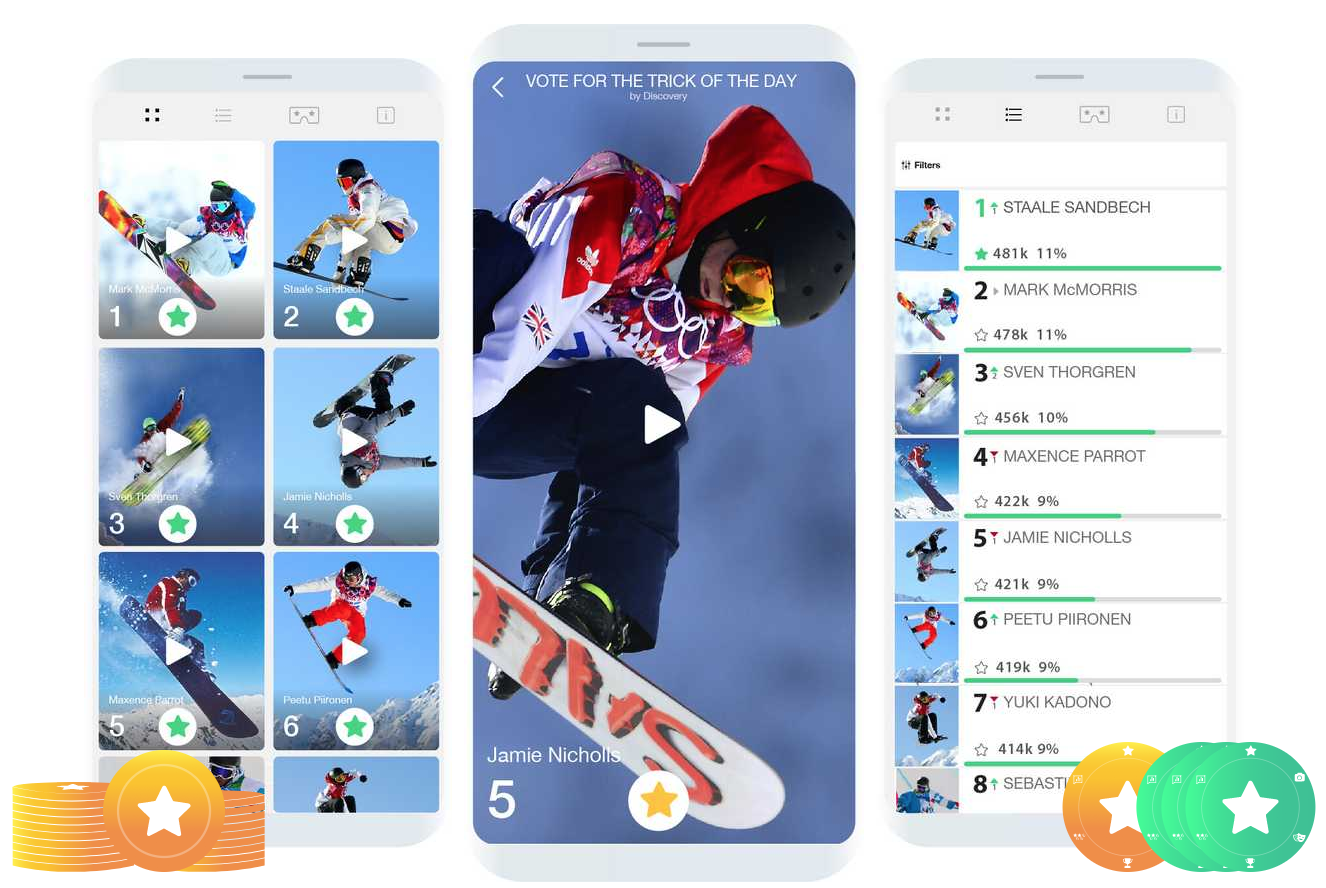
\includegraphics[width=0.6\textwidth]{images/vote_trick_of_the_day.png}
            % 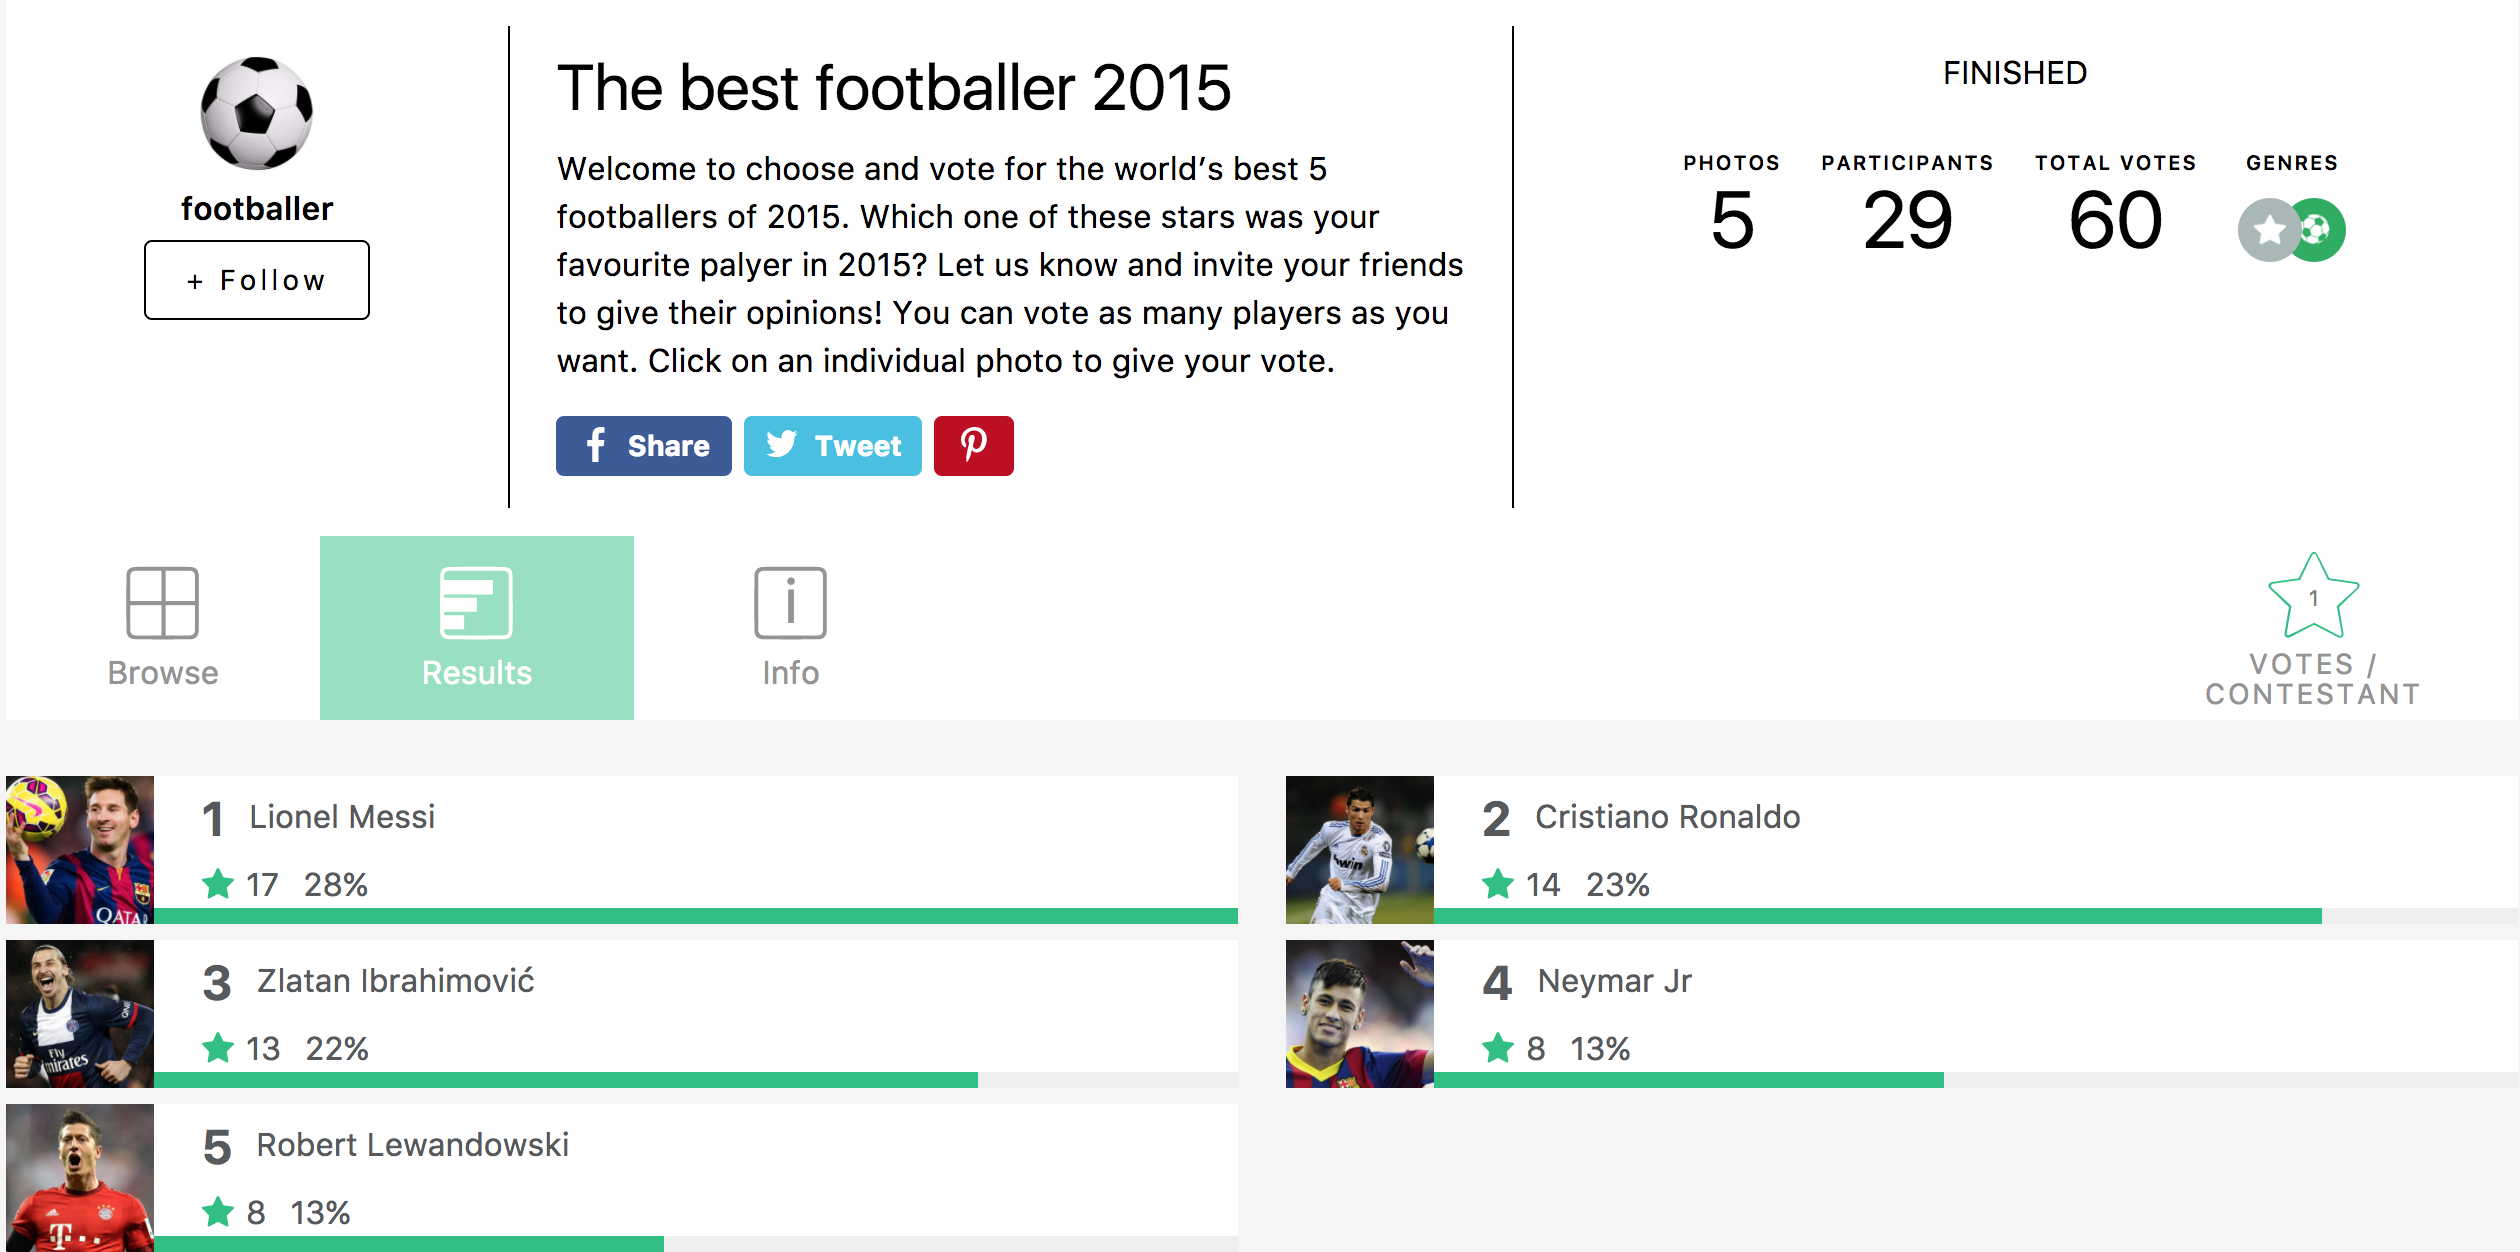
\includegraphics[width=0.6\textwidth]{images/best_footballer_2015_results.png}
            \caption{The visual appearance of a contest in Choicely.}
            \label{vote_trick_of_the_day}
        \end{center}
    \end{figure}

    The company also offers a web widget, which can be embedded as a framework in any webpage easily. The widget is often used by Choicely's customers, because it provides a convenient way to embed rich content in their own web pages, which users are already familiar with. Contests cannot be created through the widget, but users can cast votes the same way as they would on any other platforms. Figure \ref{choicely_platforms} displays the front-end interfaces which the users interact with.
    
    Users can create contests and cast votes in contest on any of these platforms. Users may vote in arbitrary number of contests. Users may vote and participate in their own contests if they like. The voting rules can limit the number of votes that users can cast in a contest as well as on individual participants. Figure \ref{vote_trick_of_the_day} displays an example how a contests may look like on a mobile device, when the user is browsing the participants. 

    \begin{figure}[h]
        \begin{center}
            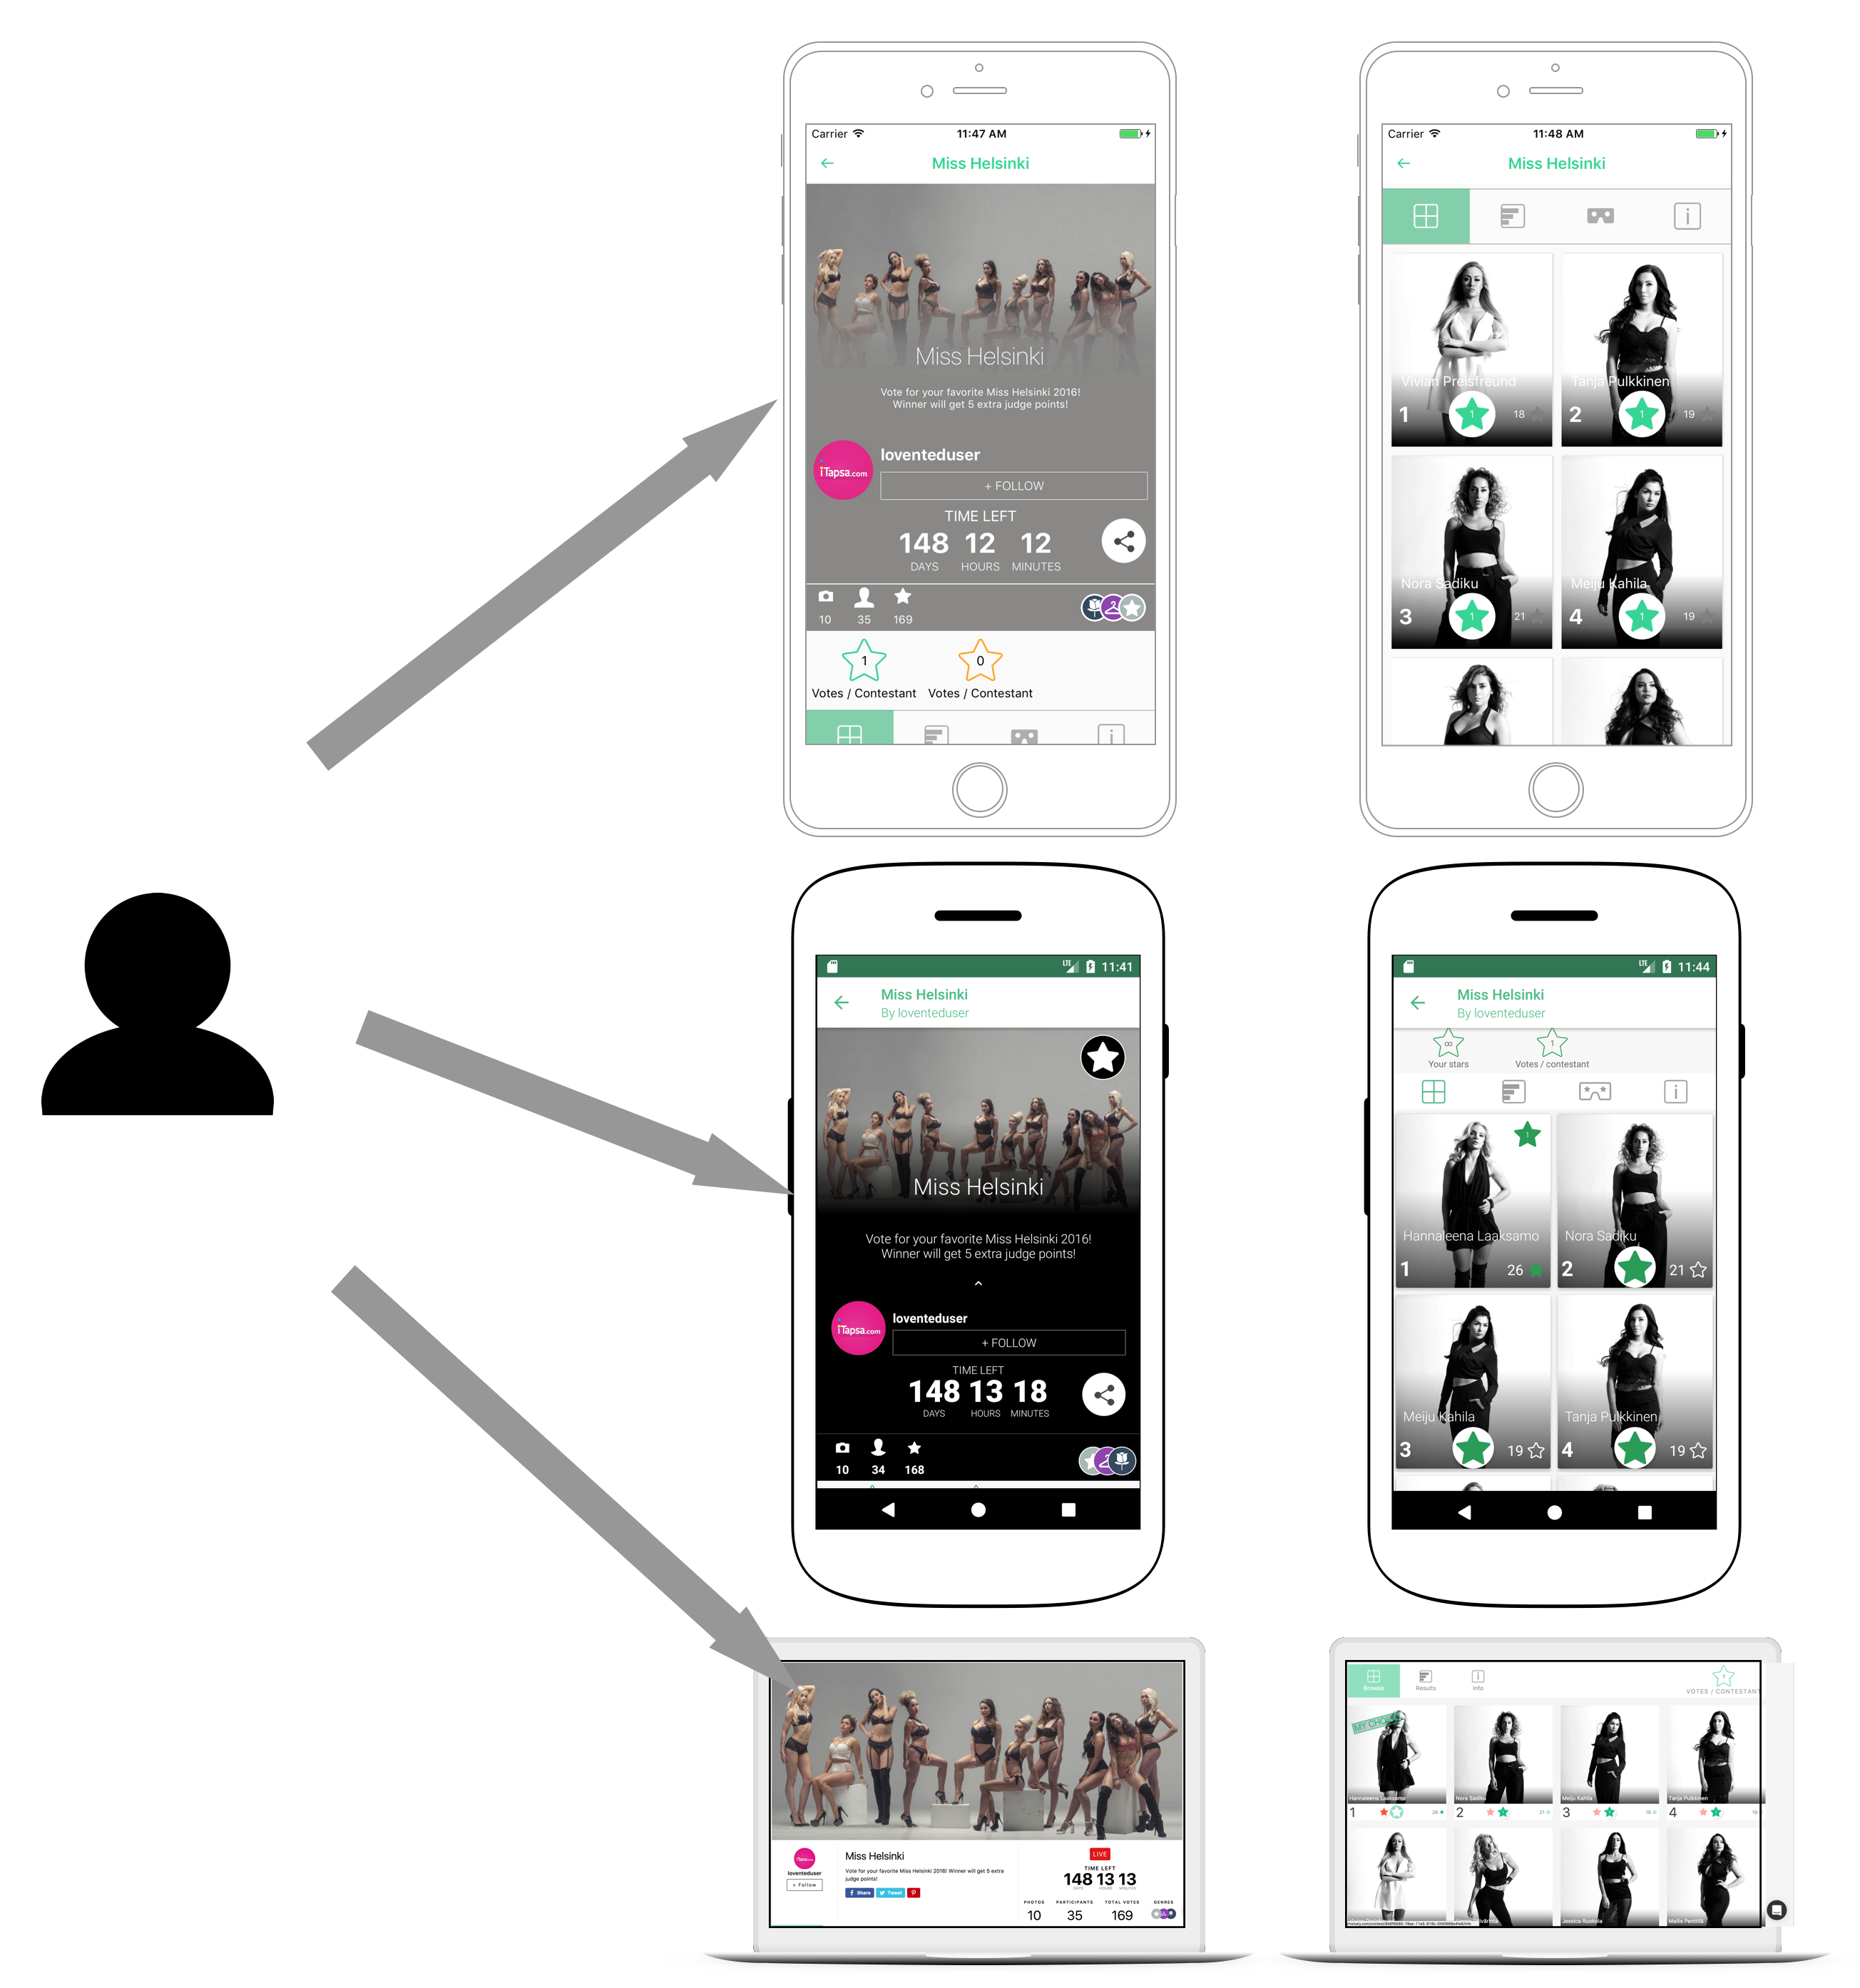
\includegraphics[width=0.6\textwidth]{images/choicely_platforms.png}
            \caption{Users can vote in contests through three interfaces: iOS devices, Android devices and web.}
            \label{choicely_platforms}
        \end{center}
    \end{figure} 

    % other contest-related data
    Contests have meta data which can facilitate data analysis. Each contest belongs to at least one but up to three of the following categories: "animals", "beauty", "danger", "design", "entertainment", "fashion", "food", "games", "humor", "sports", "travel", "other". The category labels are aligned by the contest's organizer upon creation. Contests also have starting and an ending time, between which users can vote. While votes arrive into a contest, the vote count value tells the number of total votes received, while the number of unique voters tells how many individual users have voted in the contest. Both of these values can be retrieved for individual participants as well. 

    % other contest participant-related data
    Information about contestants is limited to the contest they contend in, their names, short descriptions, image and video. As a result, that currently it is not possible to characterize contestants based on the available meta data. In other words, one of the limitations of the platform is to facilitate information about the contest participants and their traits. 
    
    % state some challenges
    There is currently no way of knowing if there is a tendency in what kind of participants tend to be more engaging to the audience. Furthermore, yet there is no possibility to know if there would be a similarity or difference in target groups behavior in terms of what kind of content they spend votes on. The goal of this thesis work from the company's perspective is to address these challenges by developing a data analysis framework that addresses these gaps. In order to perform that, a way to supplement missing piece of information from the participants images is needed, which is another aim of this work. Through the results of this study, the customers of the firm can get access to a tool, which assist them in retrospectively analyzing the engagement of their audience in the past.

\subsection{Thesis structure}
    % how is the thesis structured? 
    This chapter presents the structure of this thesis work. The next chapter explains the methodology that is chosen to address the research questions stated above. Chapter \ref{section::audience-engagement-and-user-data-analysis} presents an overview on the theoretical background and on the related work in the field of audience engagement and user data analysis. Chapter \ref{section::data-mining-at-choicely} presents the Choicely voting platform more in-depth and explains how the data analysis methods are applied at the company from a practical perspective. This section presents also the important bits and pieces that are relevant for the technical part of the study, such as the voting mechanishm, and the data structure. Chapter \ref{section::results} summarizes the results of the project at the case company. The results of are listed under subchapters by each method that was utilized. Chapter \ref{section::discussion} opens up the discussion on the results, connects the studied case to the reviewed literature, evaluates the obtained findings and derives implications from the results. This chapter is also dedicated to evaluate the chosen methods, their relevance and applicability to the problem. Finally, Chapter \ref{section::conclusions} concludes the study and points out directions for further research and development. 